\documentclass[12pt,a4paper]{article}

% ---------- Packages ----------
\usepackage{amsmath, amssymb, amsthm}
\usepackage{graphicx}
\usepackage{float}
\usepackage{geometry}
\usepackage{setspace}
\usepackage{titlesec}
\usepackage{hyperref}
\usepackage{caption}
\usepackage{subcaption}
\usepackage{booktabs}

% ---------- Page Setup ----------
\geometry{margin=1in}
\setstretch{1.25}
\titleformat{\section}{\Large\bfseries}{\thesection.}{0.5em}{}
\titleformat{\subsection}{\large\bfseries}{\thesubsection}{0.5em}{}

% ---------- Metadata ----------
\newcommand{\coursename}{ECE 712: Matrix Computations for Signal Processing}
\newcommand{\assignmenttitle}{Assignment 1}
\newcommand{\studentname}{Dai, Jiatao}
\newcommand{\studentid}{400548587}
\newcommand{\duedate}{October 12, 2025}

% ---------- Begin Document ----------
\begin{document}

% ---------- Title Page ----------
\begin{titlepage}
    \centering
    \vspace*{2cm}
    {\Huge \textbf{\assignmenttitle}}\\[1.5cm]
    {\Large \coursename}\\[1cm]
    \vspace{1cm}
    \textbf{Name:} \studentname \\[0.3cm]
    \textbf{Student ID:} \studentid \\[0.3cm]
    \textbf{Date:} \duedate \\[2cm]

    \vfill
    {\Large McMaster University \\[0.3cm]
    Department of Electrical and Computer Engineering \\[0.3cm]
    October 12, 2025}
\end{titlepage}

% ---------- Table of Contents ----------
\tableofcontents
\newpage

% ======================================================
\section{Question 1: PCA Compression and Reconstruction Error}

\subsection{Method}
In this question, we are given a $1000 \times 5$ data matrix $X$ (from \texttt{X.mat}). 
First, each column of $X$ is mean-centered to get $X_c = X - \bar{X}$. 
Then we compute the covariance matrix:
\[
C = \frac{1}{N-1} X_c^\top X_c,
\]
where $N = 1000$. 

Next, we perform eigen-decomposition of $C$:
\[
C = V \Lambda V^\top,
\]
where $\Lambda$ contains the eigenvalues and $V$ the eigenvectors. 
For a given number of components $r$, we take the first $r$ columns of $V$ as $V_r$ and project the data:
\[
Y = X_c V_r.
\]
We can then reconstruct the data (in the centered form) by
\[
\hat{X}_r = Y V_r^\top = X_c V_r V_r^\top.
\]
The reconstruction error is measured using the Frobenius norm:
\[
E(r) = \|X_c - \hat{X}_r\|_F^2.
\]
We also compute the cumulative variance explained by the first $r$ components:
\[
\text{Cumulative Variance}(r) = \frac{\sum_{i=1}^r \lambda_i}{\sum_{i=1}^5 \lambda_i}.
\]

\subsection{Results}
The PCA results from the dataset are summarized below.

\begin{itemize}
    \item Eigenvalues (sorted): $\{5.0849,\ 0.0914,\ 0.0272,\ 0.0152,\ 0.0103\}$.
    \item Cumulative variance explained (\%): $\{97.25,\ 98.99,\ 99.51,\ 99.80,\ 100.0\}$.
    \item Reconstruction error $E(r)$: $\{143.91,\ 52.59,\ 25.45,\ 10.30,\ \approx 0\}$.
\end{itemize}

\begin{table}[H]
\centering
\caption{Summary of PCA results for $r = 1$ to $5$.}
\begin{tabular}{@{}cccc@{}}
\toprule
$r$ & Eigenvalue $\lambda_r$ & Cumulative Var.\ (\%) & $E(r)$ \\
\midrule
1 & 5.0849 & 97.25 & 143.91 \\
2 & 0.0914 & 98.99 & 52.59 \\
3 & 0.0272 & 99.51 & 25.45 \\
4 & 0.0152 & 99.80 & 10.30 \\
5 & 0.0103 & 100.0 & $\approx 0$ \\
\bottomrule
\end{tabular}
\end{table}

The figures below show the reconstruction error, cumulative variance, and eigenvalue distribution.

\begin{figure}[H]
    \centering
    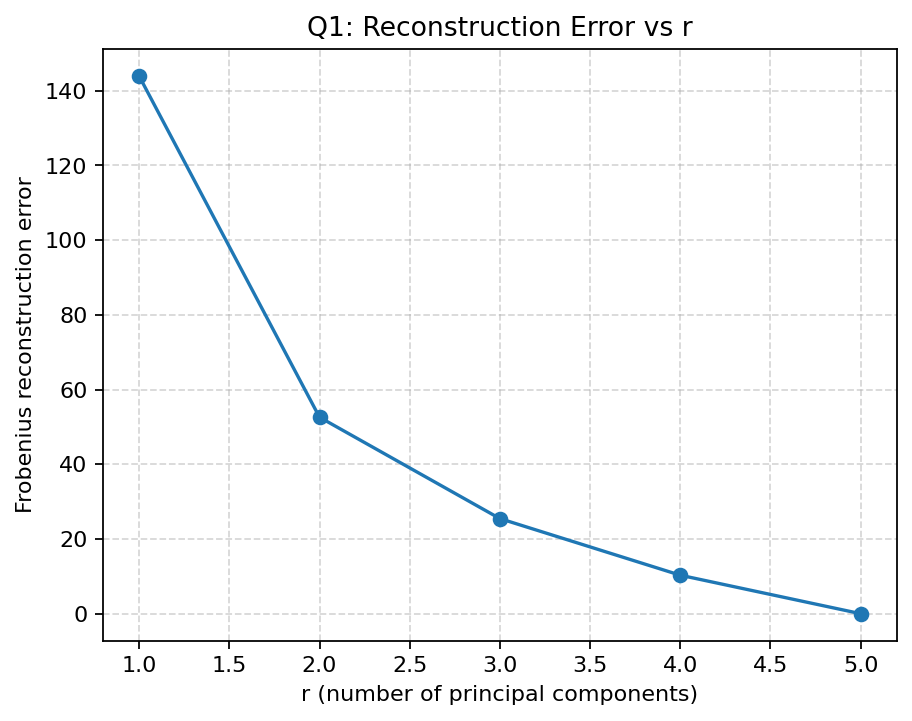
\includegraphics[width=0.75\textwidth]{outputs/q1/q1_error_vs_r.png}
    \caption{Reconstruction error vs. number of components $r$.}
\end{figure}

\begin{figure}[H]
    \centering
    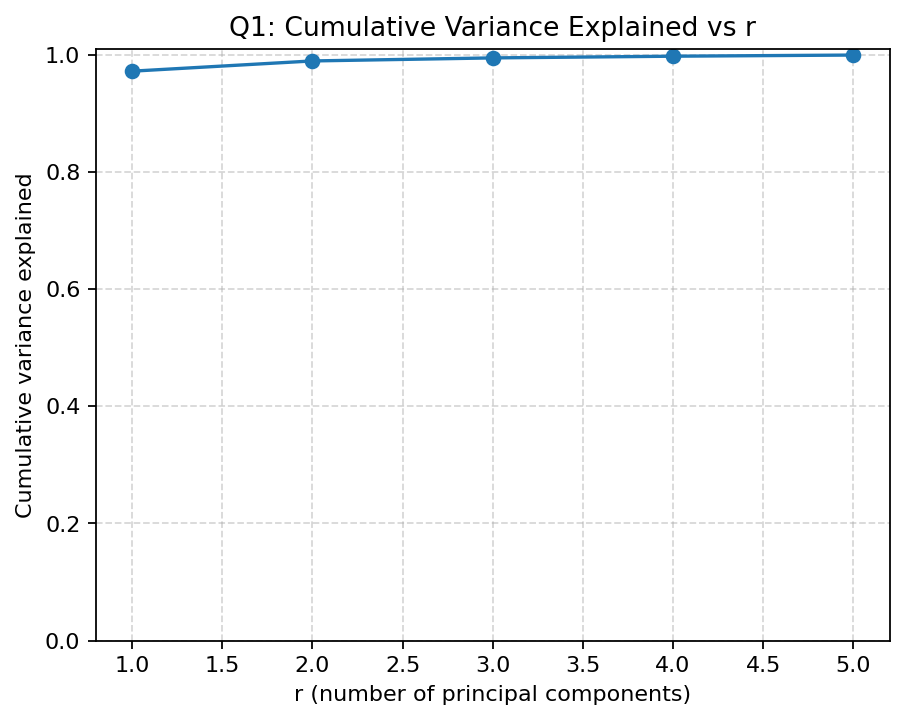
\includegraphics[width=0.75\textwidth]{outputs/q1/q1_cumvar_vs_r.png}
    \caption{Cumulative variance explained by top $r$ components.}
\end{figure}

\begin{figure}[H]
    \centering
    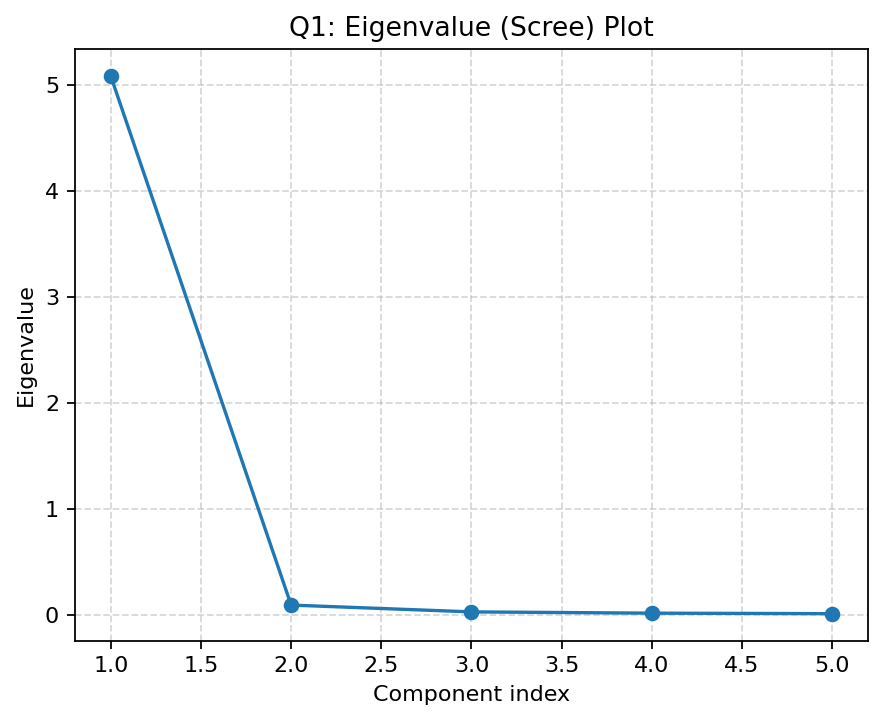
\includegraphics[width=0.75\textwidth]{outputs/q1/q1_scree.png}
    \caption{Eigenvalue (scree) plot.}
\end{figure}

\subsection{Discussion}
From the results, we can see that most of the variance (around 97\%) is already captured by the first component. 
The remaining components only add a small amount of variance. 
As $r$ increases, the reconstruction error keeps getting smaller, which makes sense since we are keeping more information.

\subsection{Conclusion}
In this dataset, using just the first principal component already keeps most of the data variation. 
If we use more components, the error decreases but the improvement becomes smaller. 
A reasonable choice is $r=1$ or $r=2$, depending on how much accuracy we need.

% ======================================================
\newpage
\section{Question 2: Proof of Minimum Reconstruction Error of PCA}

\subsection{Objective}
Let $X \in \mathbb{R}^{m\times d}$ be a mean-centered data matrix.
For any $r$-dimensional orthonormal basis $U_r \in \mathbb{R}^{d\times r}$ with $U_r^\top U_r = I_r$, 
the orthogonal projection of the data onto $\text{span}(U_r)$ and its reconstruction are
\[
\hat X_r = XU_rU_r^\top.
\]
The reconstruction error is defined as
\[
E(U_r) = \|X - \hat X_r\|_F^2 = \|X - XU_rU_r^\top\|_F^2.
\]
Our goal is to show that the PCA basis $U_r$ gives the smallest possible reconstruction error among all orthonormal bases.

\subsection{Proof (Projection $\Rightarrow$ Trace Maximization $\Rightarrow$ PCA)}
Because $P_{U_r}=U_rU_r^\top$ is an orthogonal projector, we have
\[
\|X\|_F^2 = \|XP_{U_r}\|_F^2 + \|X(I-P_{U_r})\|_F^2
\quad\Rightarrow\quad
E(U_r) = \|X\|_F^2 - \|XU_rU_r^\top\|_F^2.
\]
Thus, minimizing $E(U_r)$ is the same as maximizing $\|XU_r\|_F^2$.
Since
\[
\|XU_r\|_F^2 = \text{tr}(U_r^\top X^\top XU_r),
\]
we want to find $U_r$ that makes this trace as large as possible.

Let $X^\top X = V\Lambda V^\top$ be the eigen-decomposition with eigenvalues
$\lambda_1 \ge \lambda_2 \ge \cdots \ge \lambda_d$.
From the properties of symmetric matrices, the maximum trace is obtained when
$U_r$ is made of the first $r$ eigenvectors of $X^\top X$:
\[
U_r = [v_1,\ldots,v_r].
\]
In that case,
\[
\text{tr}(U_r^\top X^\top XU_r) = \sum_{i=1}^{r}\lambda_i.
\]
Therefore, projecting onto these eigenvectors (the PCA subspace) gives the smallest possible reconstruction error.

\subsection{Conclusion}
PCA provides the orthogonal basis that minimizes the reconstruction error,
and the minimum possible error is
\[
E_{\min}(r) = \sum_{i=r+1}^{d} \sigma_i^2,
\]
where $\sigma_i$ are the singular values of $X$.
This result matches what we observed in Question~1, where the reconstruction error decreases as $r$ increases.

% ======================================================
\newpage
\section{Question 3: Minimum-Variance FIR Filter Design}

\subsection{Objective}
In this question, we are given a mean-centered coloured random sequence $x[n]$ (from \texttt{xb.mat}).  
The goal is to design a finite impulse response (FIR) filter $h[n]$ with length $N$ and unit norm $\|h\|_2 = 1$ so that the output $y[n]=(h*x)[n]$ has the smallest possible variance.

\subsection{Method}
First, we calculate the sample autocorrelation $r_x[\ell]$ of $x[n]$.  
Then we form a Toeplitz covariance matrix
\[
R_x = \mathrm{Toeplitz}(r_x[0], r_x[1], \ldots, r_x[N-1]).
\]
The output variance can be written as
\[
\sigma_y^2 = h^\top R_x h, \quad \text{subject to } \|h\|_2 = 1.
\]
The minimum variance happens when $h$ is the eigenvector of $R_x$ that corresponds to its smallest eigenvalue.  
In other words, we just find the smallest eigenvalue and take the corresponding eigenvector as the filter.

\subsection{Implementation}
The Python script \texttt{q3\_minvar\_fir\_final.py} loads the signal, computes $r_x[\ell]$, builds $R_x$, and finds the minimum-variance filter for $N=8,12,16,24$.  
It also saves the plots:
\begin{itemize}
    \item \texttt{q3\_autocorr.png}: autocorrelation of $x[n]$
    \item \texttt{q3\_var\_vs\_N.png}: output variance vs.\ $N$
    \item \texttt{q3\_impulse\_N\{N\}.png}: impulse response of $h[n]$
    \item \texttt{q3\_spectrum\_N\{N\}.png}: magnitude spectrum $|H(e^{j\omega})|$
\end{itemize}

\subsection{Results}
The input signal clearly has correlation (it is not white noise), which can be seen in Fig.~\ref{fig:q3_autocorr}.  
As the filter length $N$ increases, the output variance becomes smaller (see Fig.~\ref{fig:q3_var_vs_N}).  
The quantitative results are listed in Table~\ref{tab:q3_results}.

\begin{figure}[H]
    \centering
    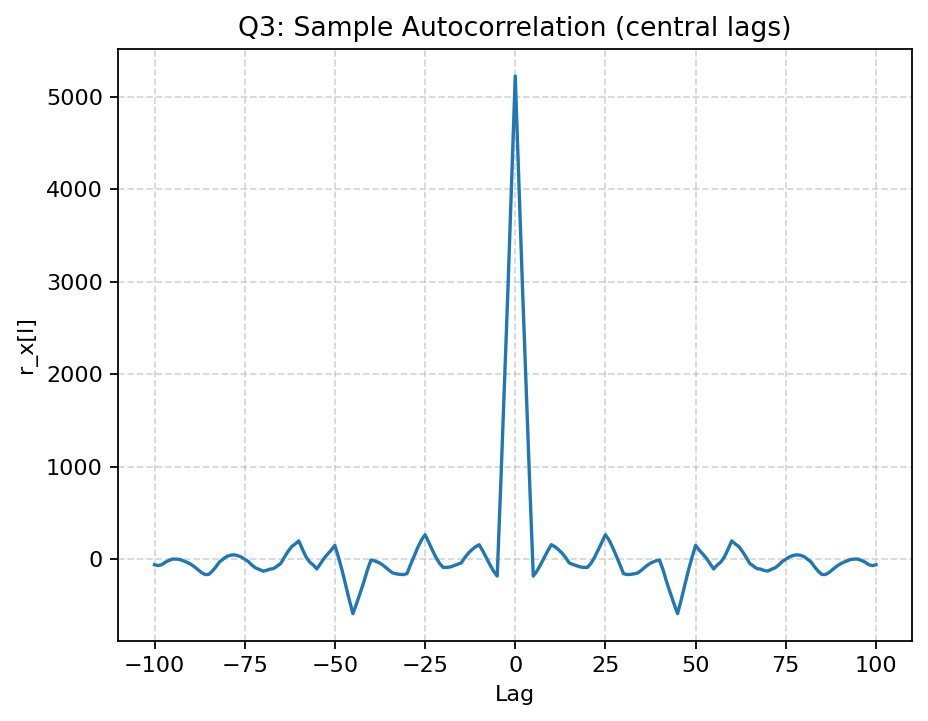
\includegraphics[width=0.7\textwidth]{outputs/q3/q3_autocorr.png}
    \caption{Autocorrelation of $x[n]$.}
    \label{fig:q3_autocorr}
\end{figure}

\begin{figure}[H]
    \centering
    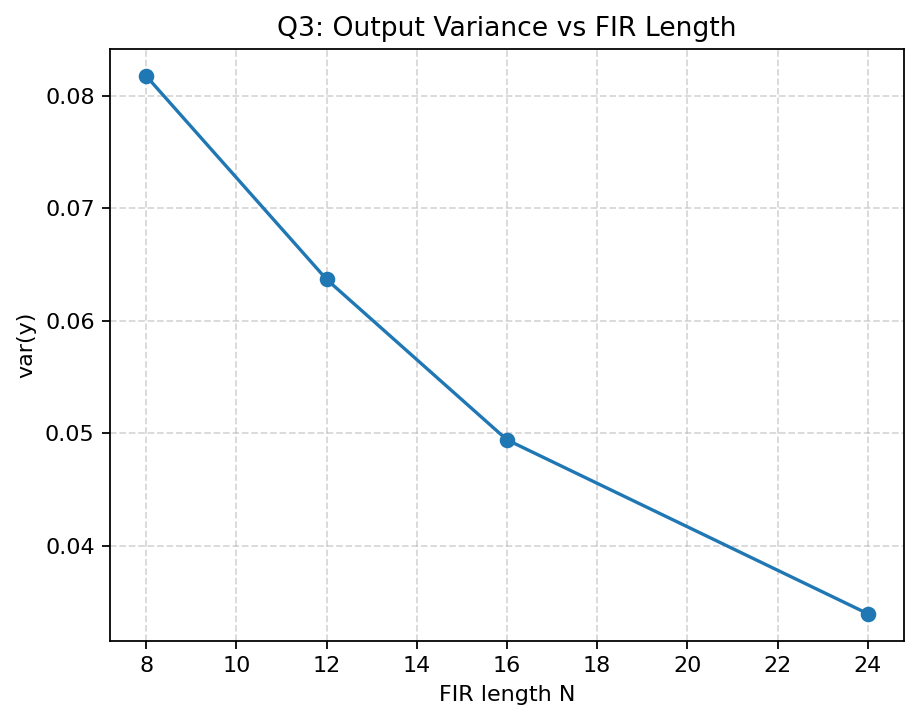
\includegraphics[width=0.7\textwidth]{outputs/q3/q3_var_vs_N.png}
    \caption{Output variance $\sigma_y^2$ vs.\ filter length $N$.}
    \label{fig:q3_var_vs_N}
\end{figure}

\begin{table}[H]
\centering
\caption{Result summary for different FIR lengths.}
\label{tab:q3_results}
\begin{tabular}{@{}ccc@{}}
\toprule
$N$ & $\sigma_y^2$ (variance) & $\lambda_{\min}(R_x)$ \\
\midrule
8  & 0.0817 & 409.53 \\
12 & 0.0637 & 318.93 \\
16 & 0.0494 & 247.38 \\
24 & 0.0340 & 170.04 \\
\bottomrule
\end{tabular}
\end{table}

Some example impulse and magnitude responses are shown in Fig.~\ref{fig:q3_impulse_spectrum}.  
When $N$ is larger, the filter becomes smoother and can reduce more of the correlated part of the signal.

\begin{figure}[H]
    \centering
    \begin{subfigure}{0.48\textwidth}
        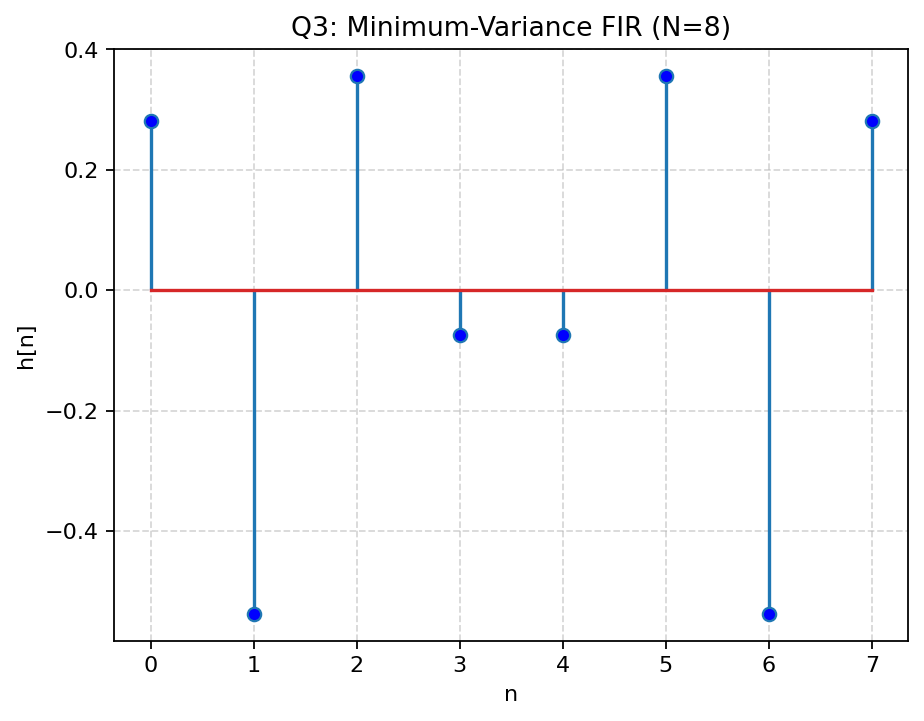
\includegraphics[width=\linewidth]{outputs/q3/N8/q3_impulse_N8.png}
        \caption{$h[n]$ for $N=8$}
    \end{subfigure}\hfill
    \begin{subfigure}{0.48\textwidth}
        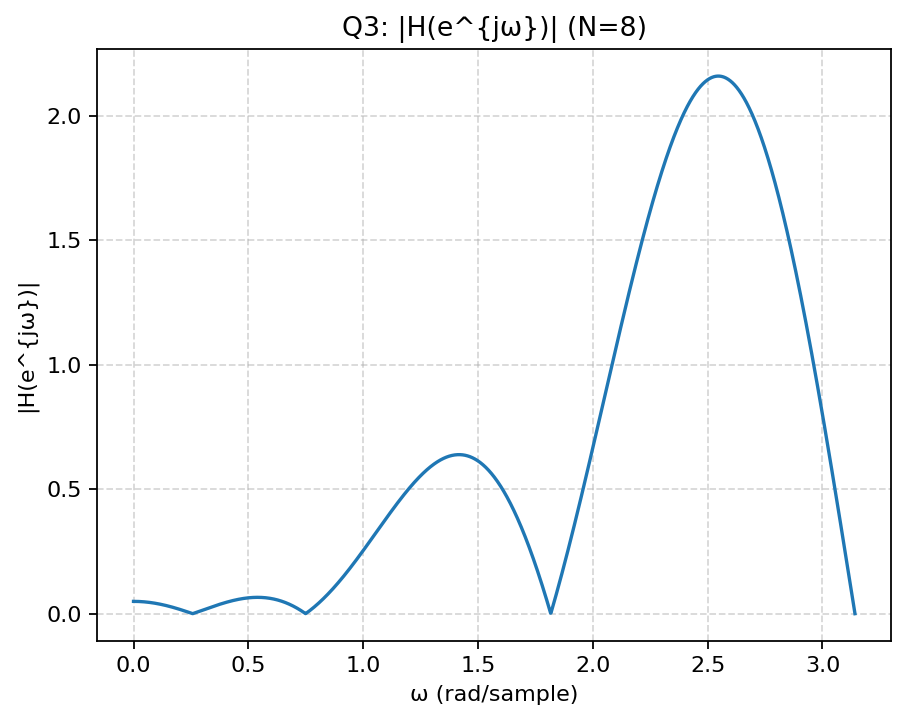
\includegraphics[width=\linewidth]{outputs/q3/N8/q3_spectrum_N8.png}
        \caption{$|H(e^{j\omega})|$ for $N=8$}
    \end{subfigure}\\[0.6em]
    \begin{subfigure}{0.48\textwidth}
        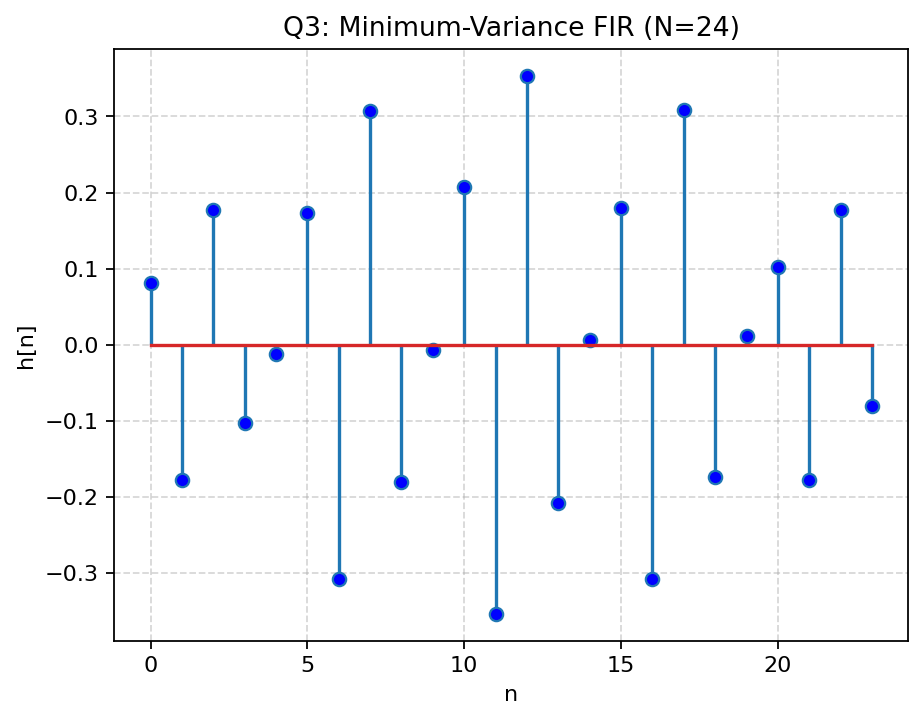
\includegraphics[width=\linewidth]{outputs/q3/N24/q3_impulse_N24.png}
        \caption{$h[n]$ for $N=24$}
    \end{subfigure}\hfill
    \begin{subfigure}{0.48\textwidth}
        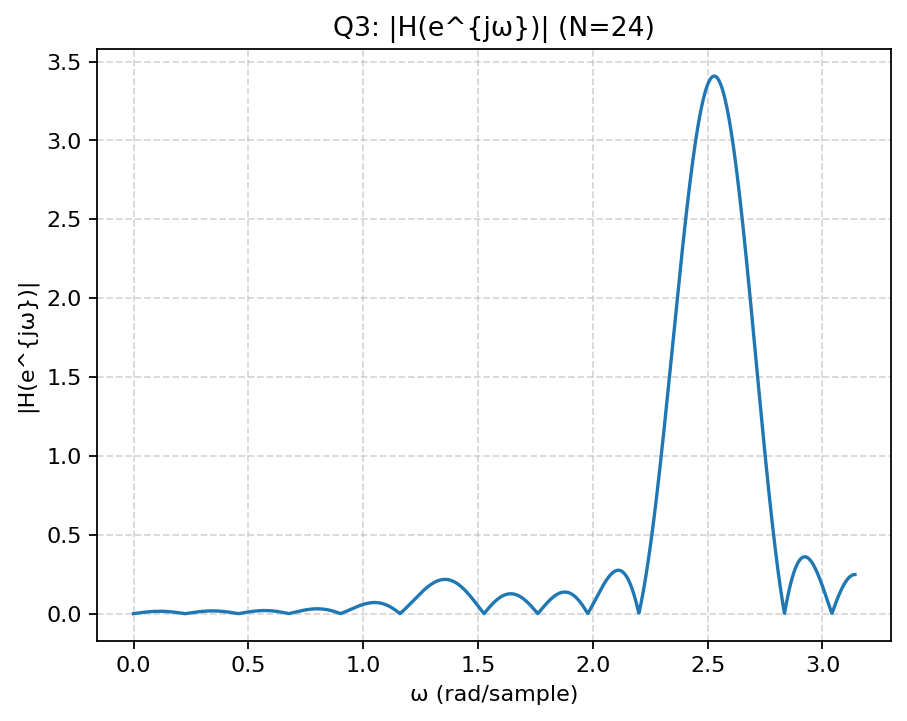
\includegraphics[width=\linewidth]{outputs/q3/N24/q3_spectrum_N24.png}
        \caption{$|H(e^{j\omega})|$ for $N=24$}
    \end{subfigure}
    \caption{Impulse and magnitude responses for two filter lengths.}
    \label{fig:q3_impulse_spectrum}
\end{figure}

\subsection{Discussion and Conclusion}
From the table and plots, we can see that as $N$ increases, the filter can make the output smoother and the variance smaller.  
This matches the idea that a longer filter has more freedom to cancel out the correlation in $x[n]$.  
All the results follow the theory that the minimum-variance filter corresponds to the smallest eigenvector of $R_x$.  
In summary, the experiment confirms that the eigen-decomposition of the covariance matrix can be used to design such filters, and the implementation works as expected.
% ======================================================
\newpage
\section*{References}
\begin{itemize}
    \item J. Reilly, \textit{Fundamentals of Linear Algebra for Signal Processing}, Lecture Notes, ECE 712, McMaster University.
\end{itemize}

\end{document}